\section{2\textsuperscript{nd} Lecture: 9. Nov 2020}

\subsection{Adaptive Filters}

\subsubsection{Principle Structure of an Adaptive Filter}

- No matter what type of parameters we put into the filter, this will always be stable.

\begin{figure}[H]
	\centering
	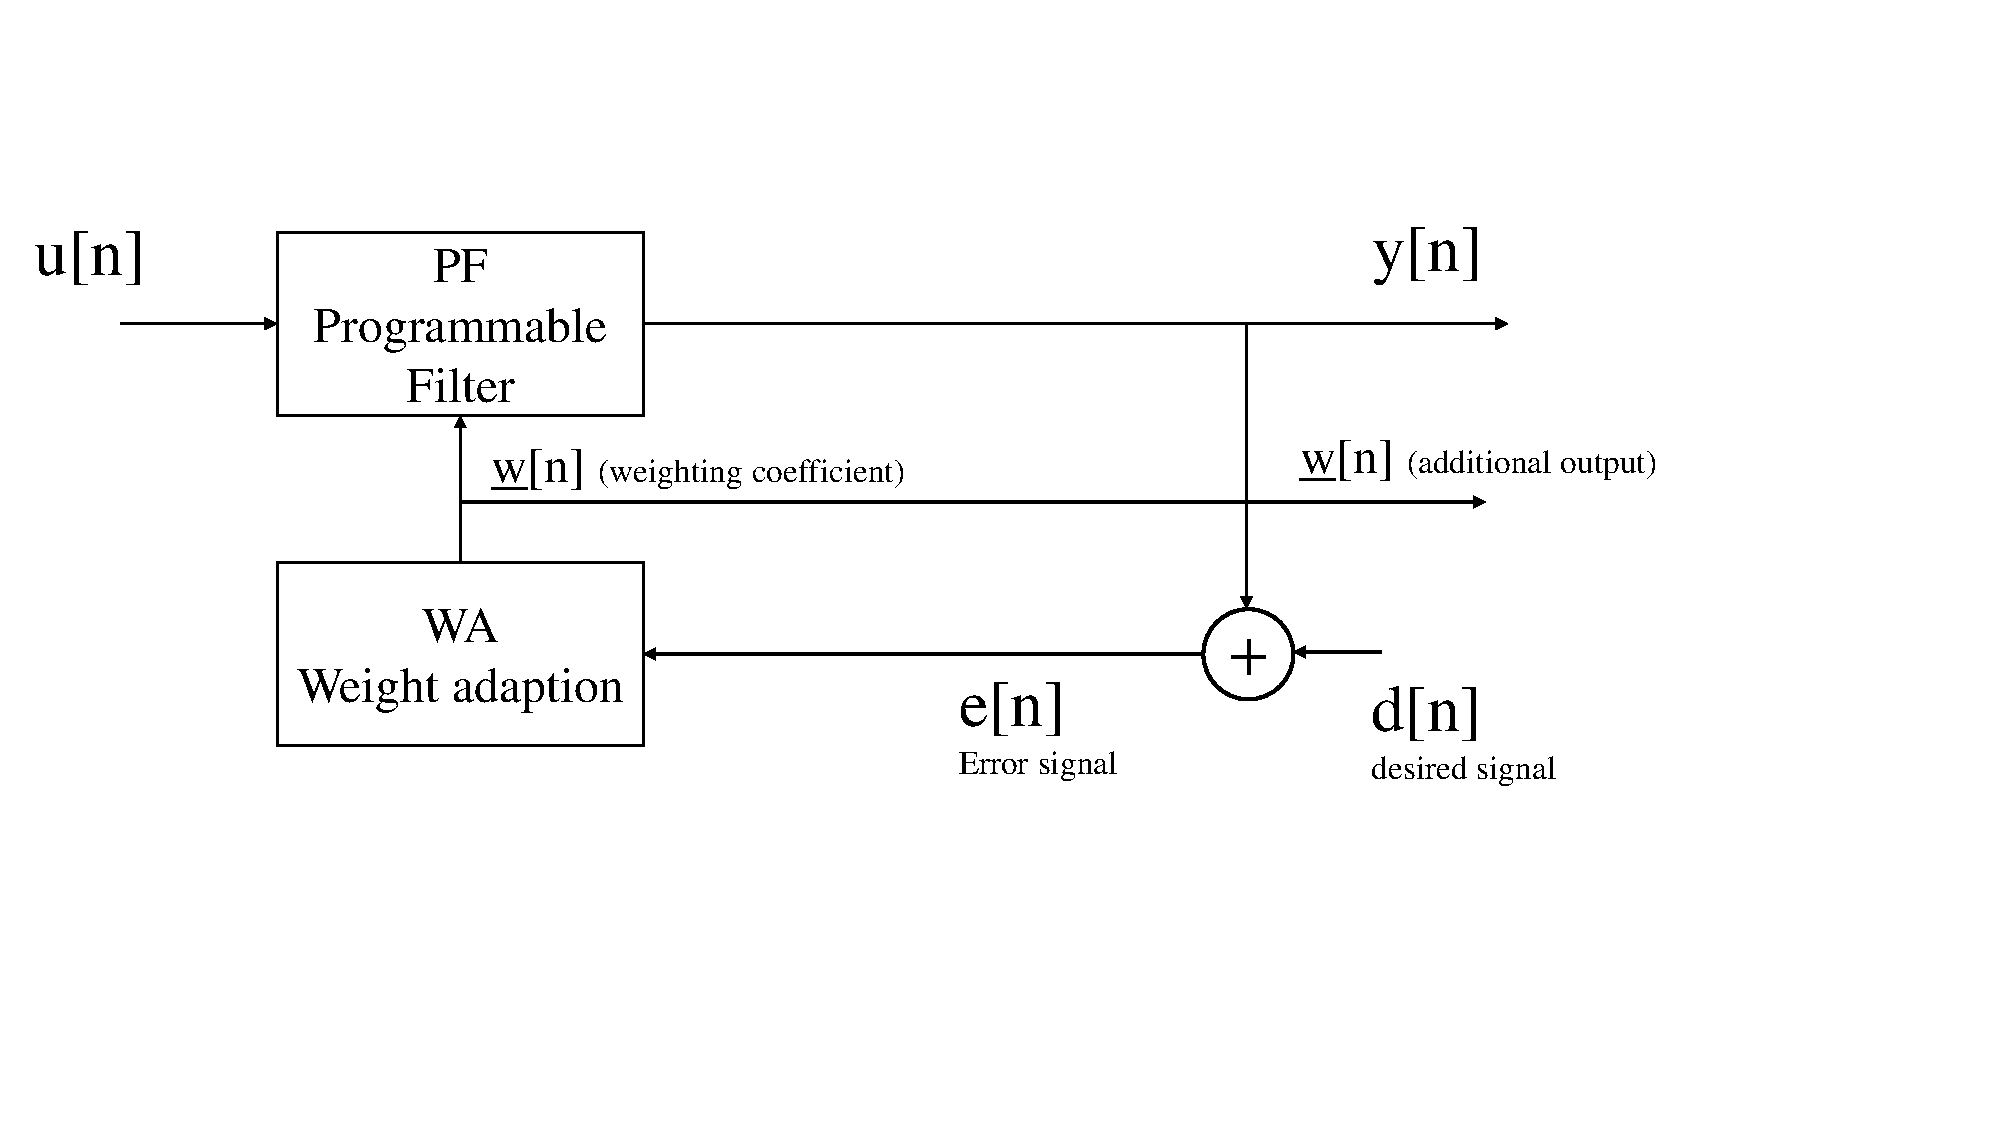
\includegraphics[scale=0.5, trim=0cm 5.5cm 0cm 3cm, clip]{adaptive_filter.pdf}
	\caption{Principle structure of an Adaptive Filter}
	\label{adaptive_filter} 
\end{figure}


$e[n] = 0 \pfeil \underline{w} [n+1] = \underline{w} [n]$\\

- An adaptive filter is composed by two things:\\
\null\qquad 1.- Programmable Filter\\
\null\qquad 2.- Weight adaptation\\

\subsection{Classes of Adaptive Filters}
\textit{...or: What are the applications of Adaptive Filters? Adaptive Filters are used for...}

\subsubsection{Filter Identification} 
	\begin{figure}[H]
		\centering
		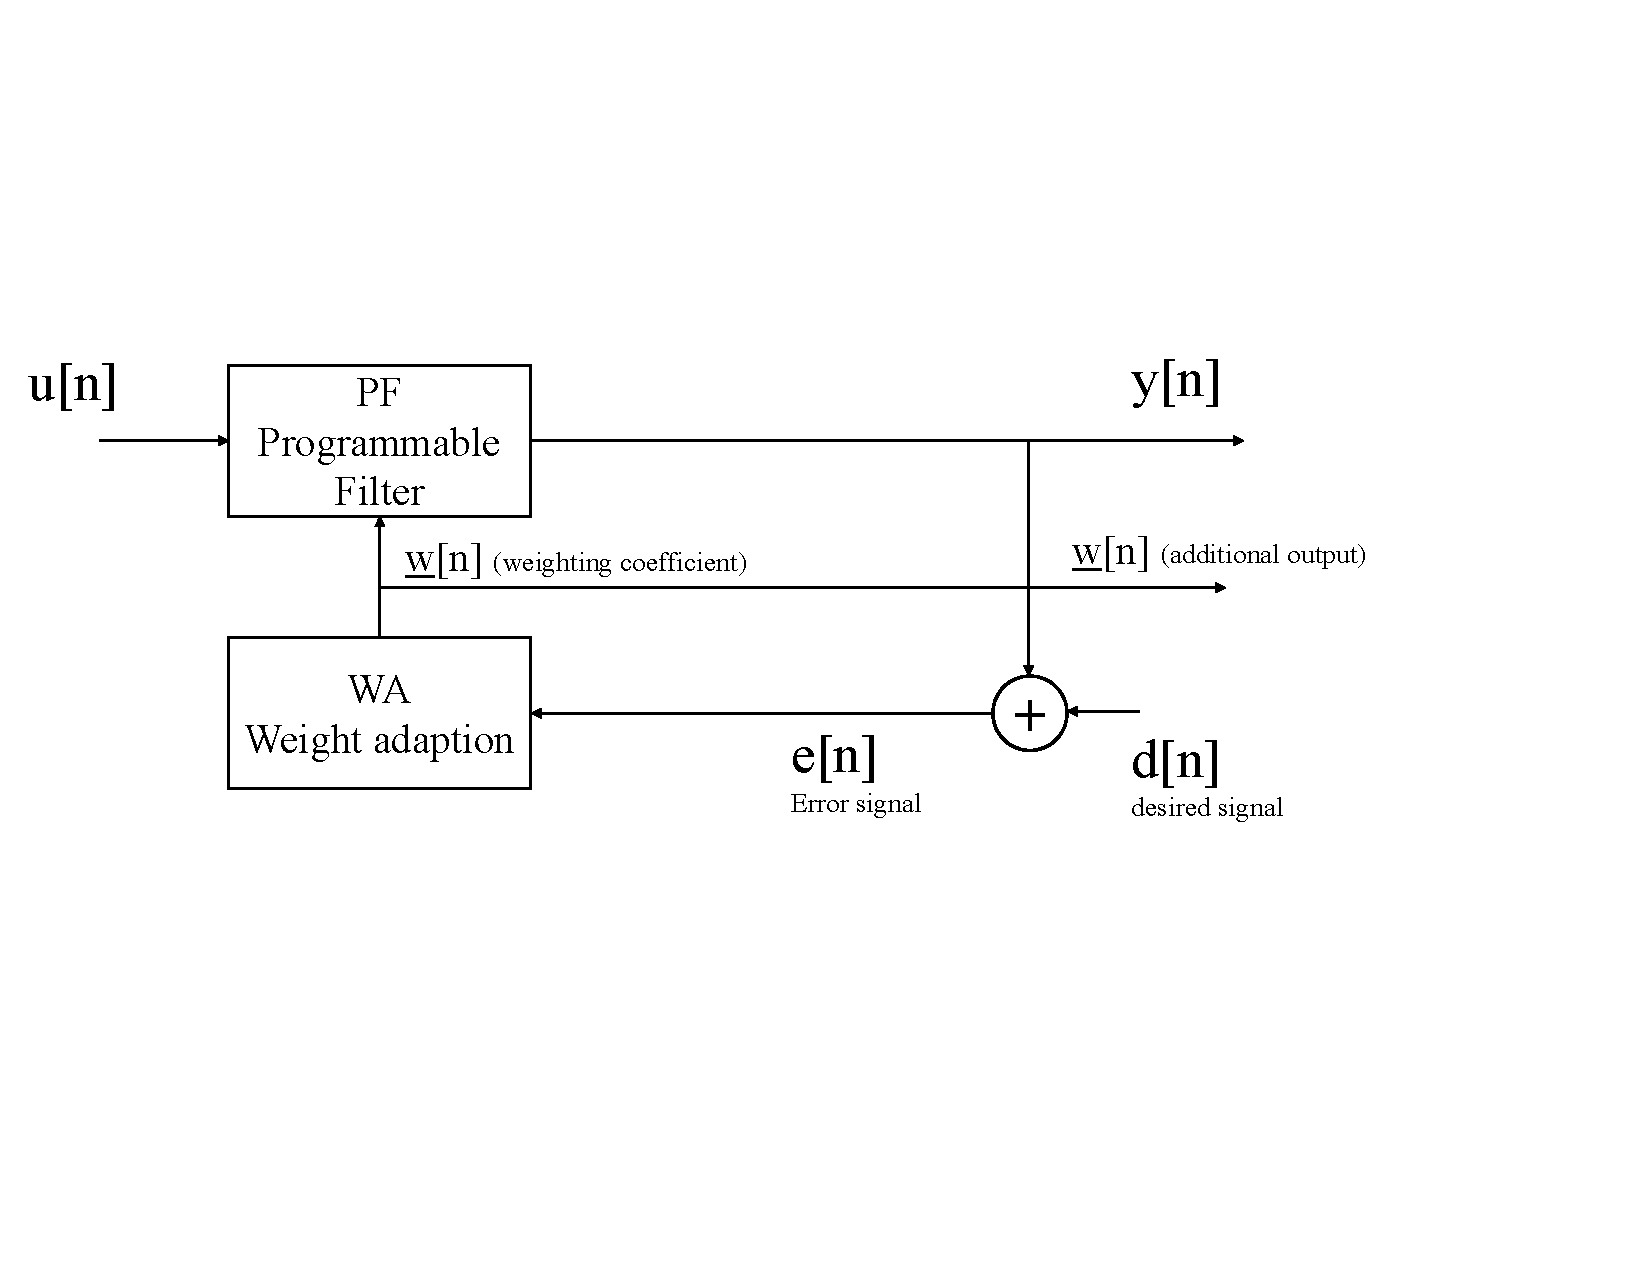
\includegraphics[scale=0.5, trim=0cm 5cm 0cm 5cm, clip]{system_identification.pdf}
		\caption{System identification}
		\label{system_identification} 
	\end{figure}

-> The weight \underline{w} is here what we really care about.


\subsubsection{System Inversion}
\begin{figure}[H]
	\centering
	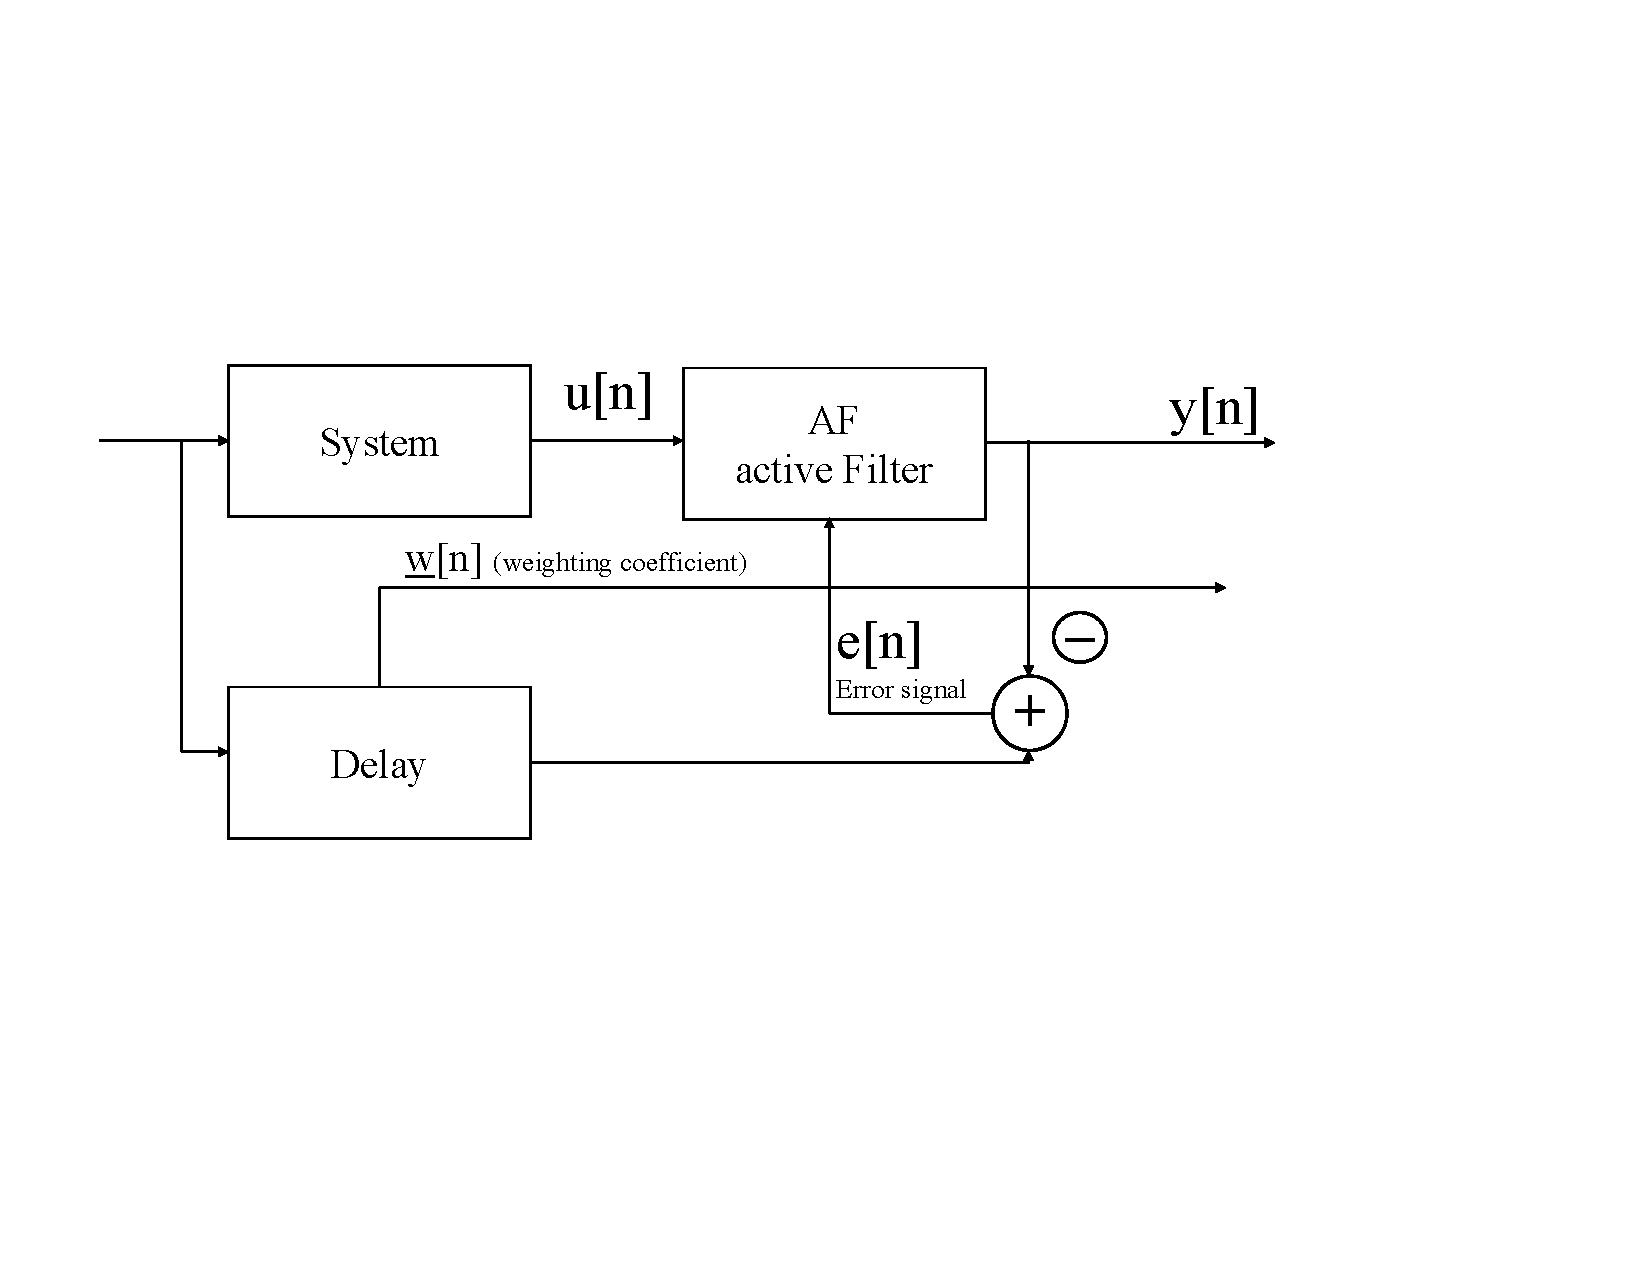
\includegraphics[scale=0.5, trim=0cm 7cm 0cm 5cm, clip]{inverse_modelling.pdf}
	\caption{Inverse Modelling}
	\label{inversemodelling} 
\end{figure}

- The delay is there to give more time to the AF to predict the output. 

\subsubsection{Prediction}
\begin{figure}[H]
	\centering
	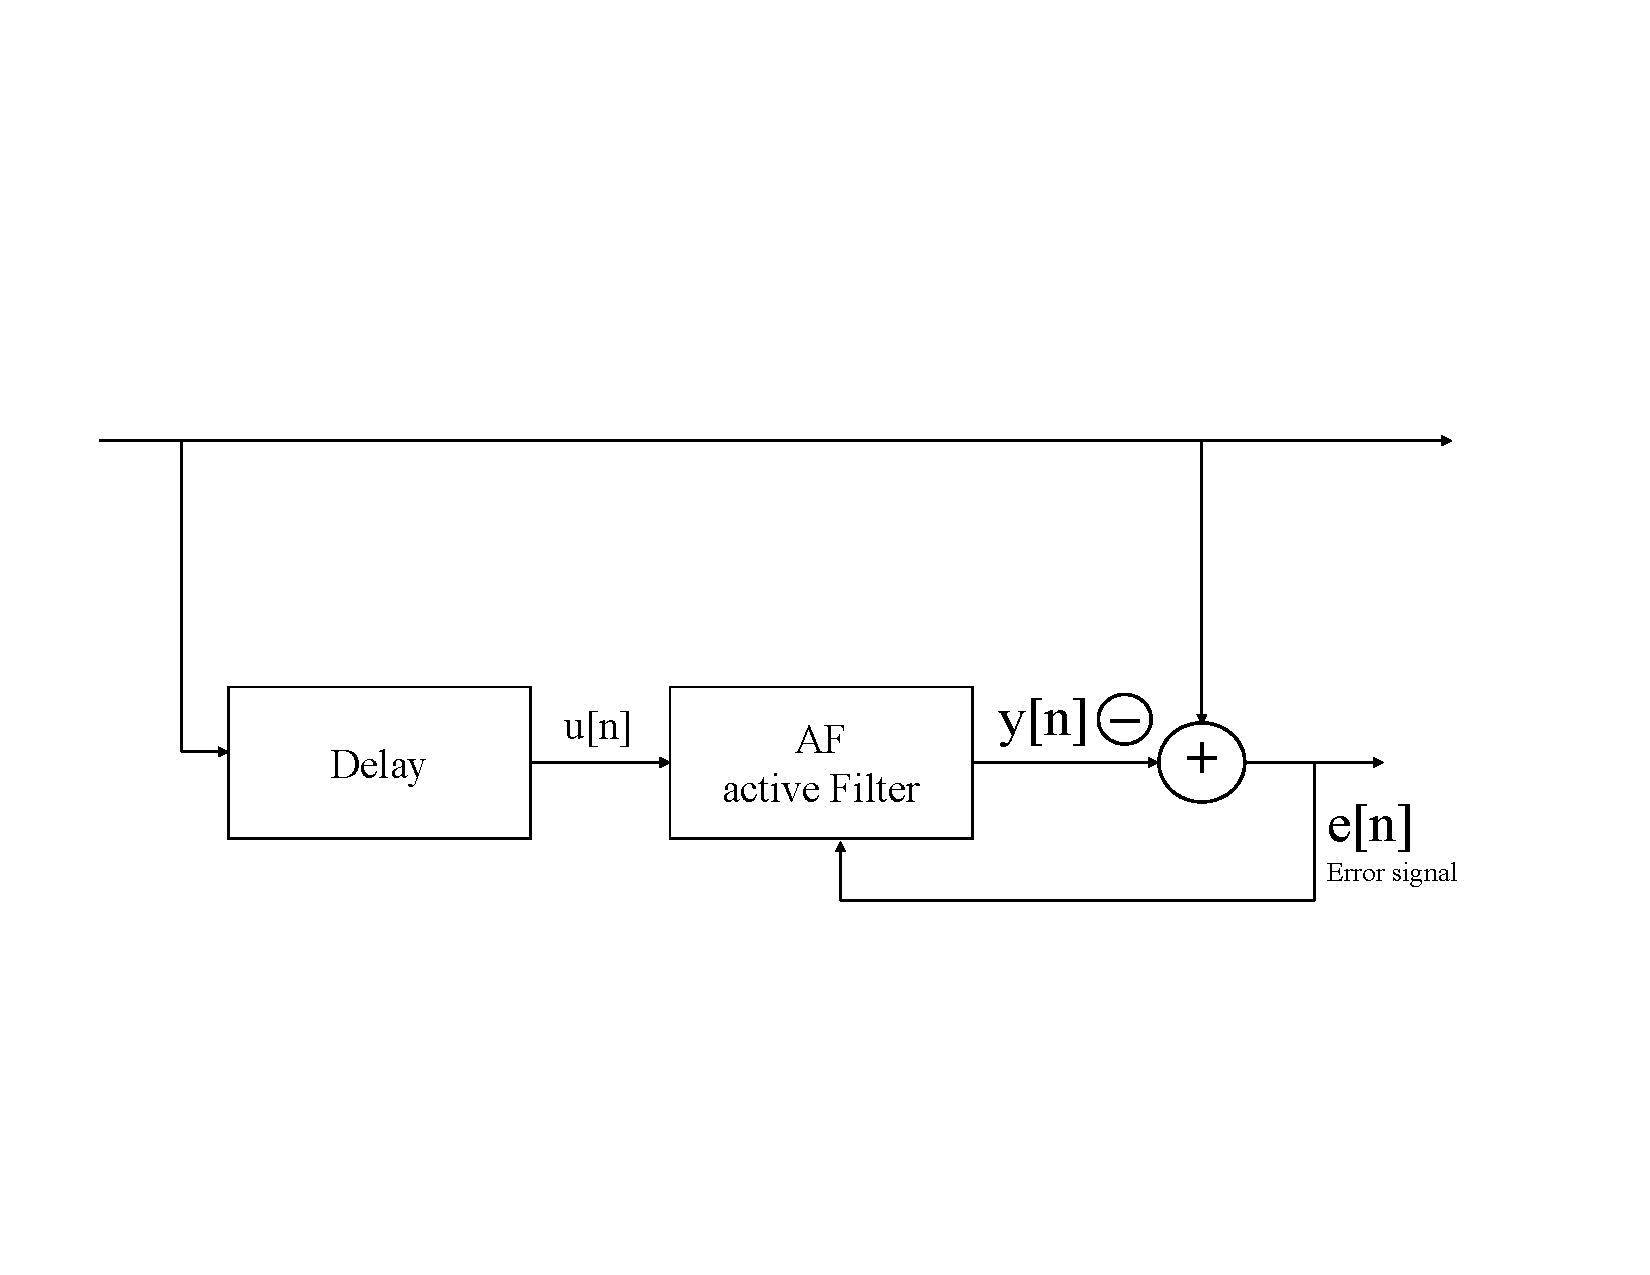
\includegraphics[scale=0.5, trim=0cm 4cm 0cm 5cm, clip]{prediction.pdf}
	\caption{Prediction}
	\label{prediction} 
\end{figure}

Out of the past - we can predict the \textit{present}. 

We run into trouble if the error signal $e[n]$ is quantized. Therefore, we introduce a compressor and a decompressor. 

\begin{figure}[H]
	\centering
	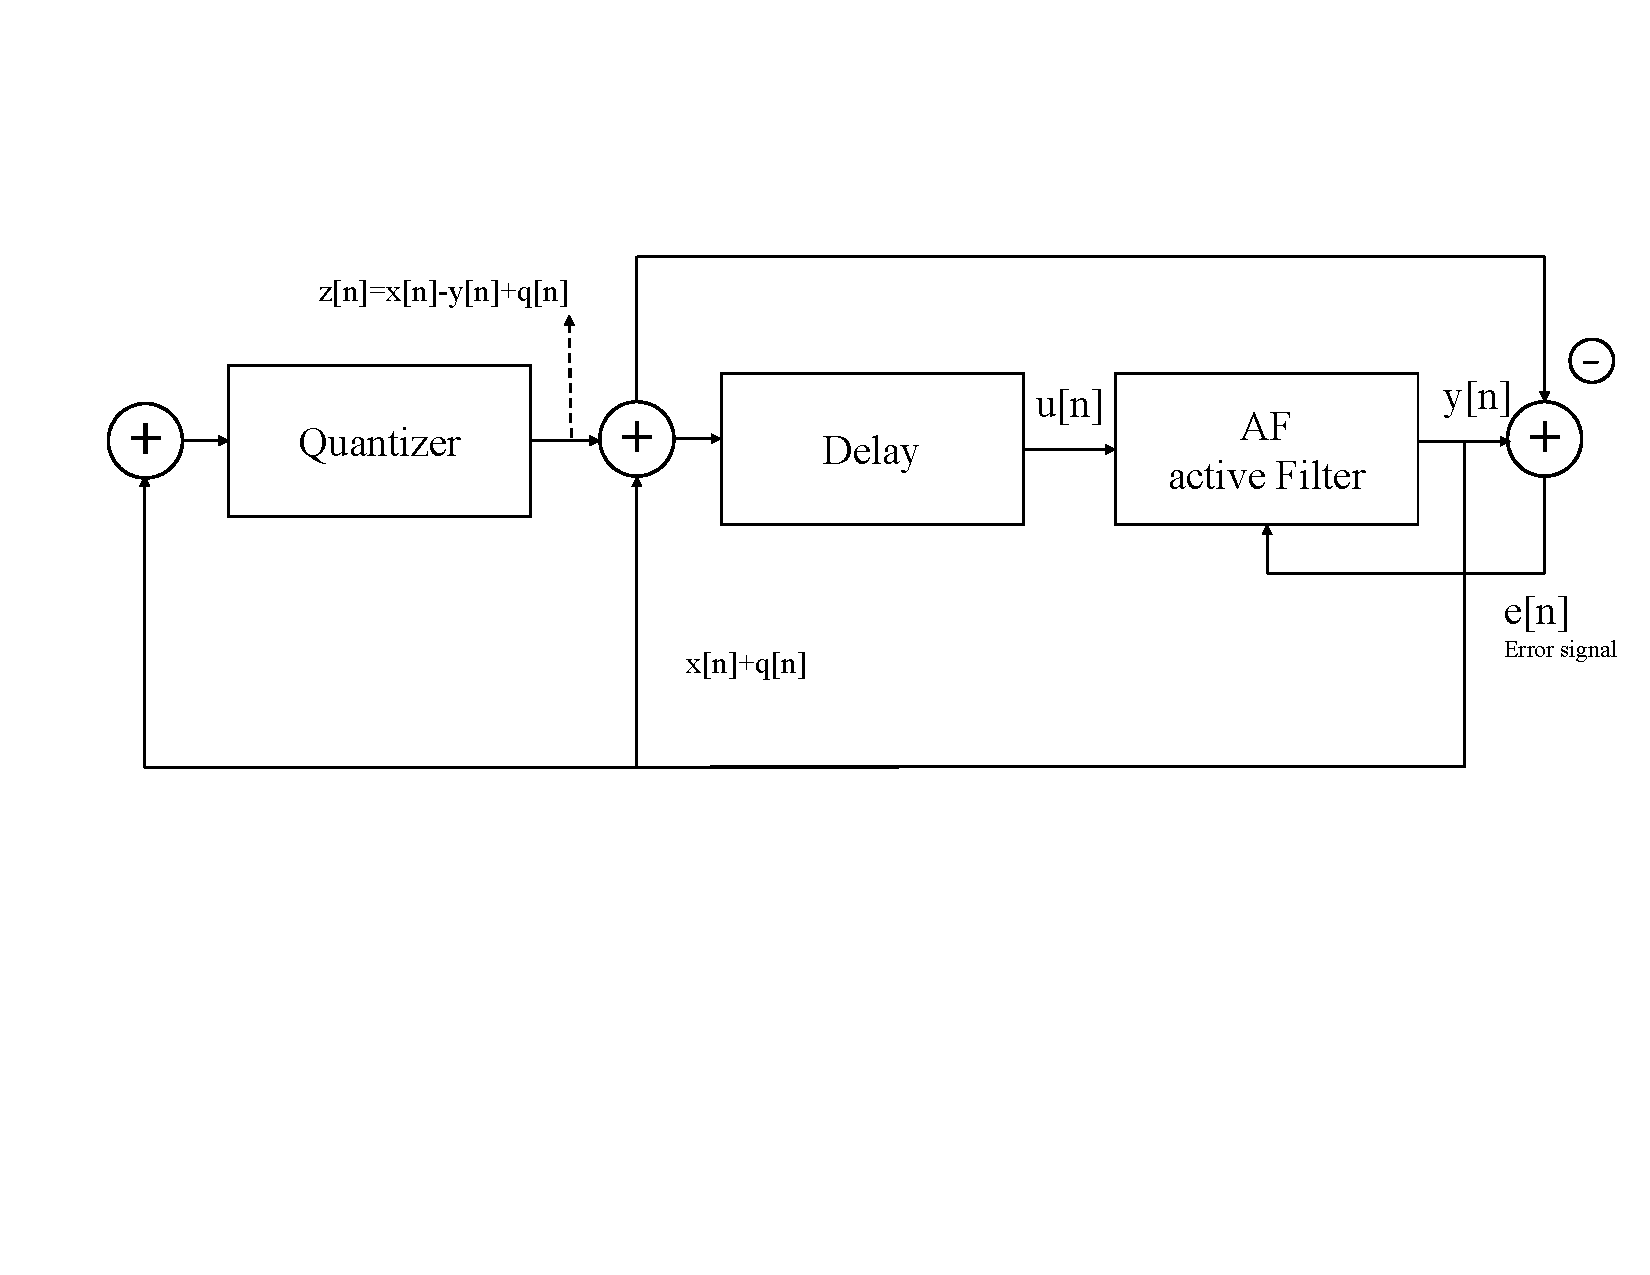
\includegraphics[scale=0.65, trim=0cm 7cm 0cm 3cm, clip]{compressor.pdf}
	\caption{Compressor}
	\label{compressor} 
\end{figure}

Predictive filter works well \pfeil if error is small\\

\begin{figure}[H]
	\centering
	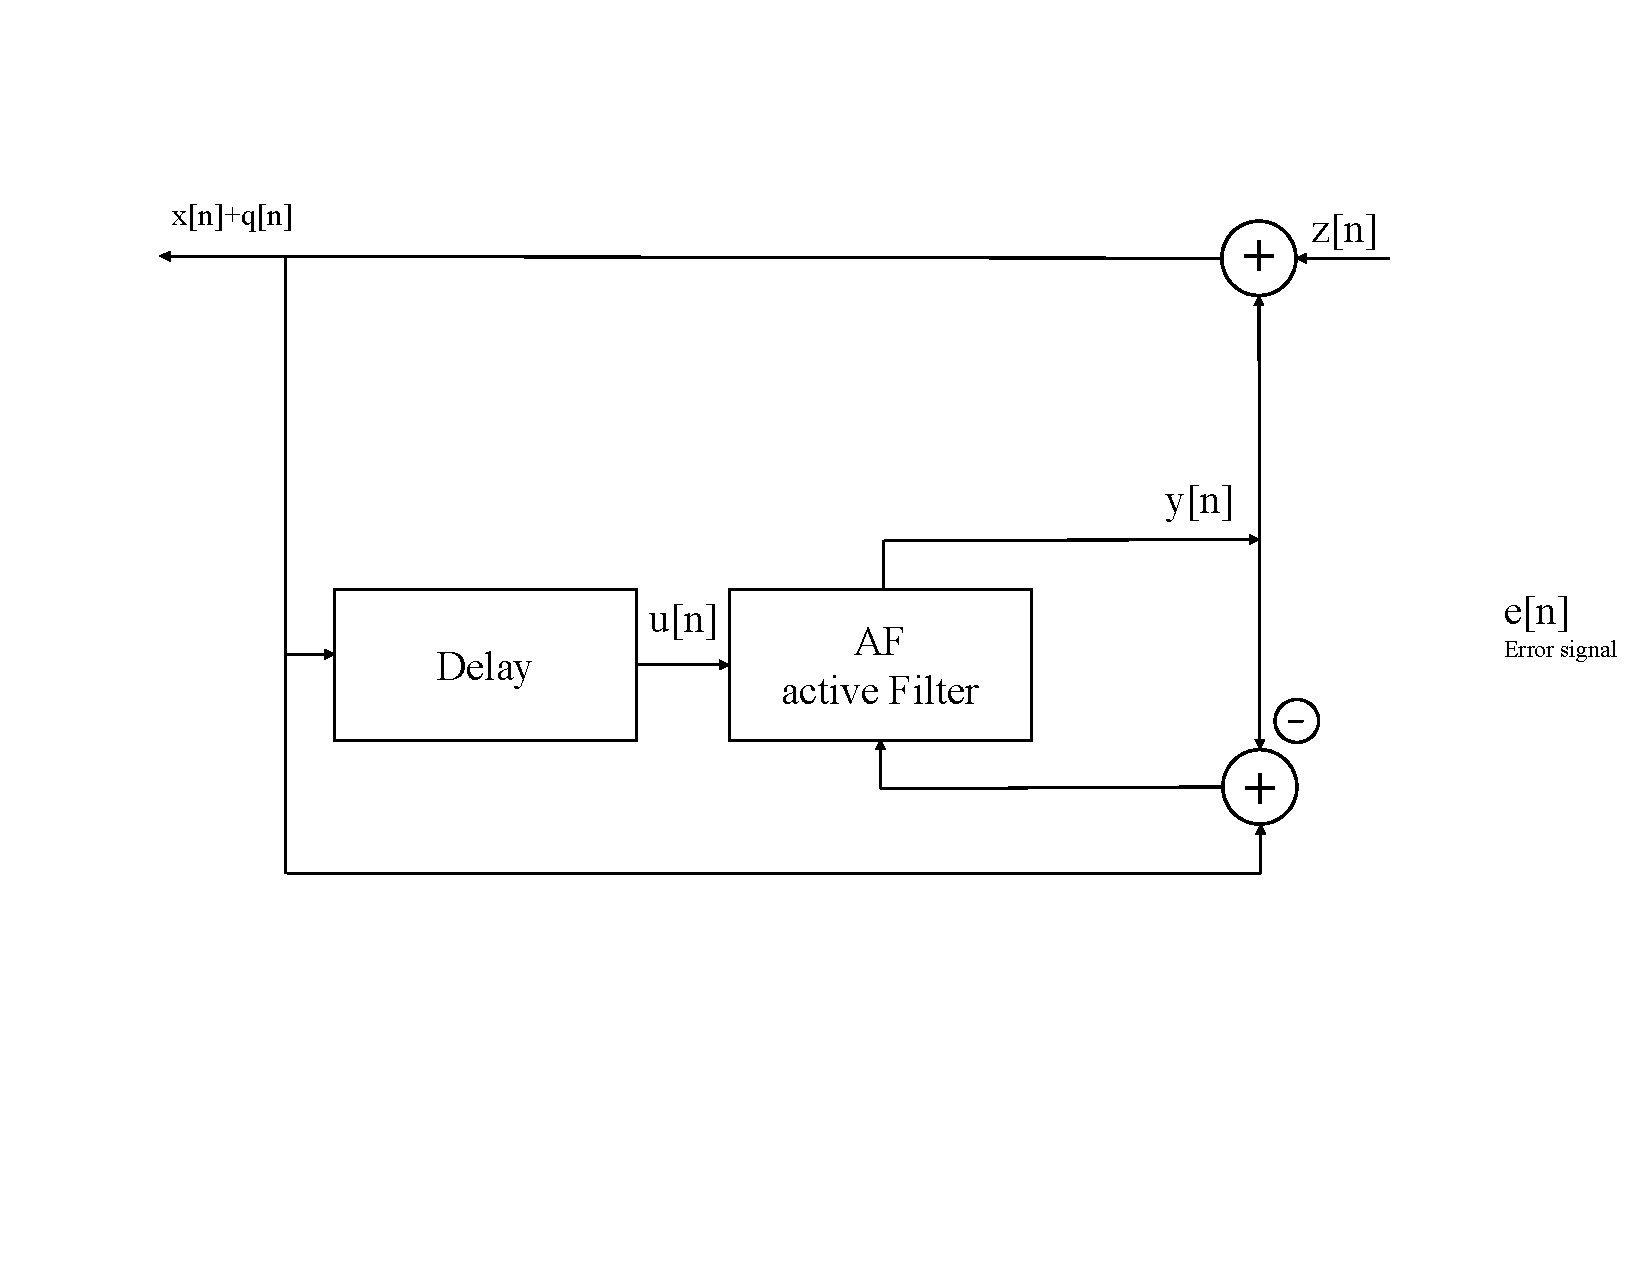
\includegraphics[scale=0.65, trim=0cm 5cm 0cm 2cm, clip]{decompressor.pdf}
	\caption{Decompressor}
	\label{decompressor} 
\end{figure}

Thanks to this type Adaptive Filter, signals can be compressed to certain bit-amount (\textit{e.g.: how many bits do we need to compress a voice signal in order for it to still be audible?})\\

\pfeil plot y-Axis:=$e[n]$\\
\pfeil plot x-Axis:=$num_bits$\\ 

-> You search for compromiss. The smaller the error, the better the predictive filter.


\subsubsection{Interference Cancellation}

\begin{figure}[H]
	\centering
	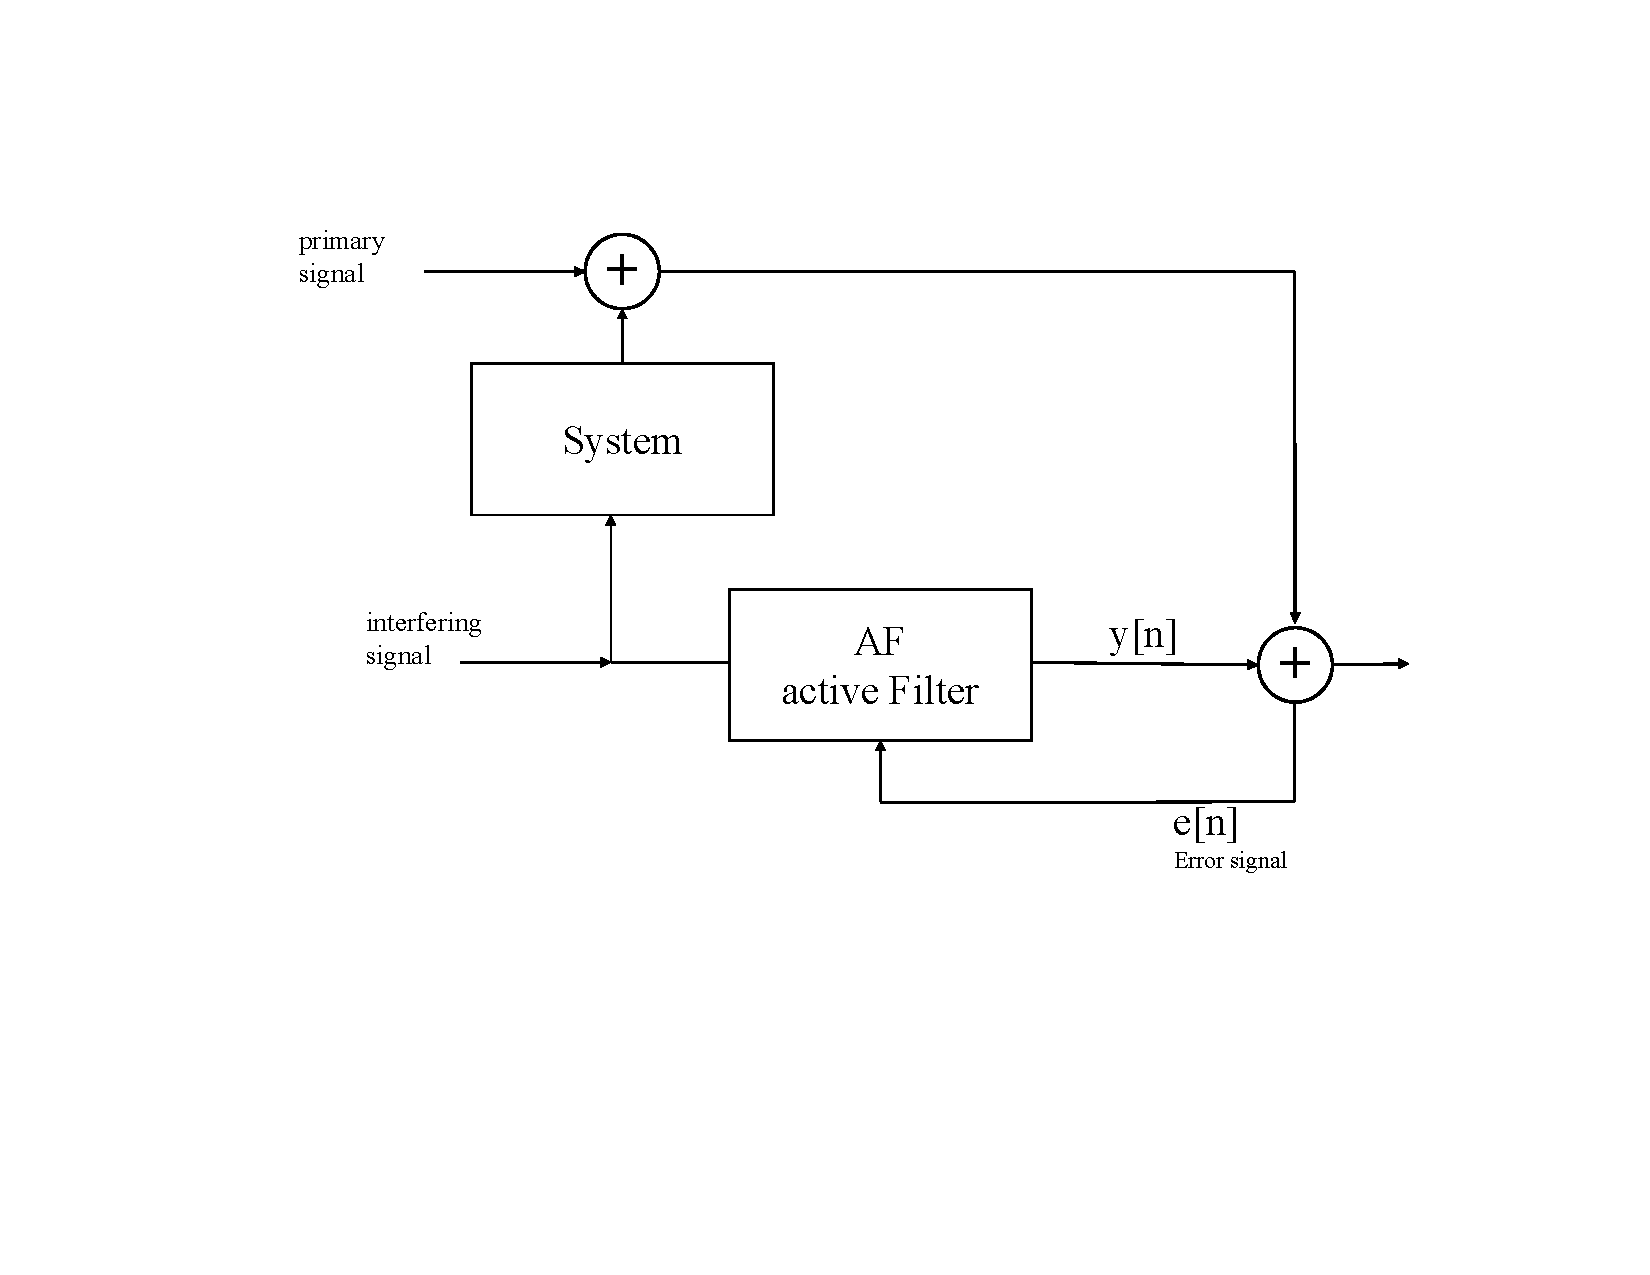
\includegraphics[scale=0.65, trim=0cm 6cm 0cm 3cm, clip]{interference_chanellation.pdf}
	\caption{Interference Cancellation}
	\label{interference1} 
\end{figure}

Assume primary signal and interfering signal are statistically independent. A linear filter can in this case separate the primary signal from the sumated signal. A good adaptive filter can also crack the signals if the signals are statisctically dependent. 

This can be ilustrated in the example of a person listening to music (noise) over speakers and speaking to a microphone at the same time. 

\begin{figure}[H]
	\centering
	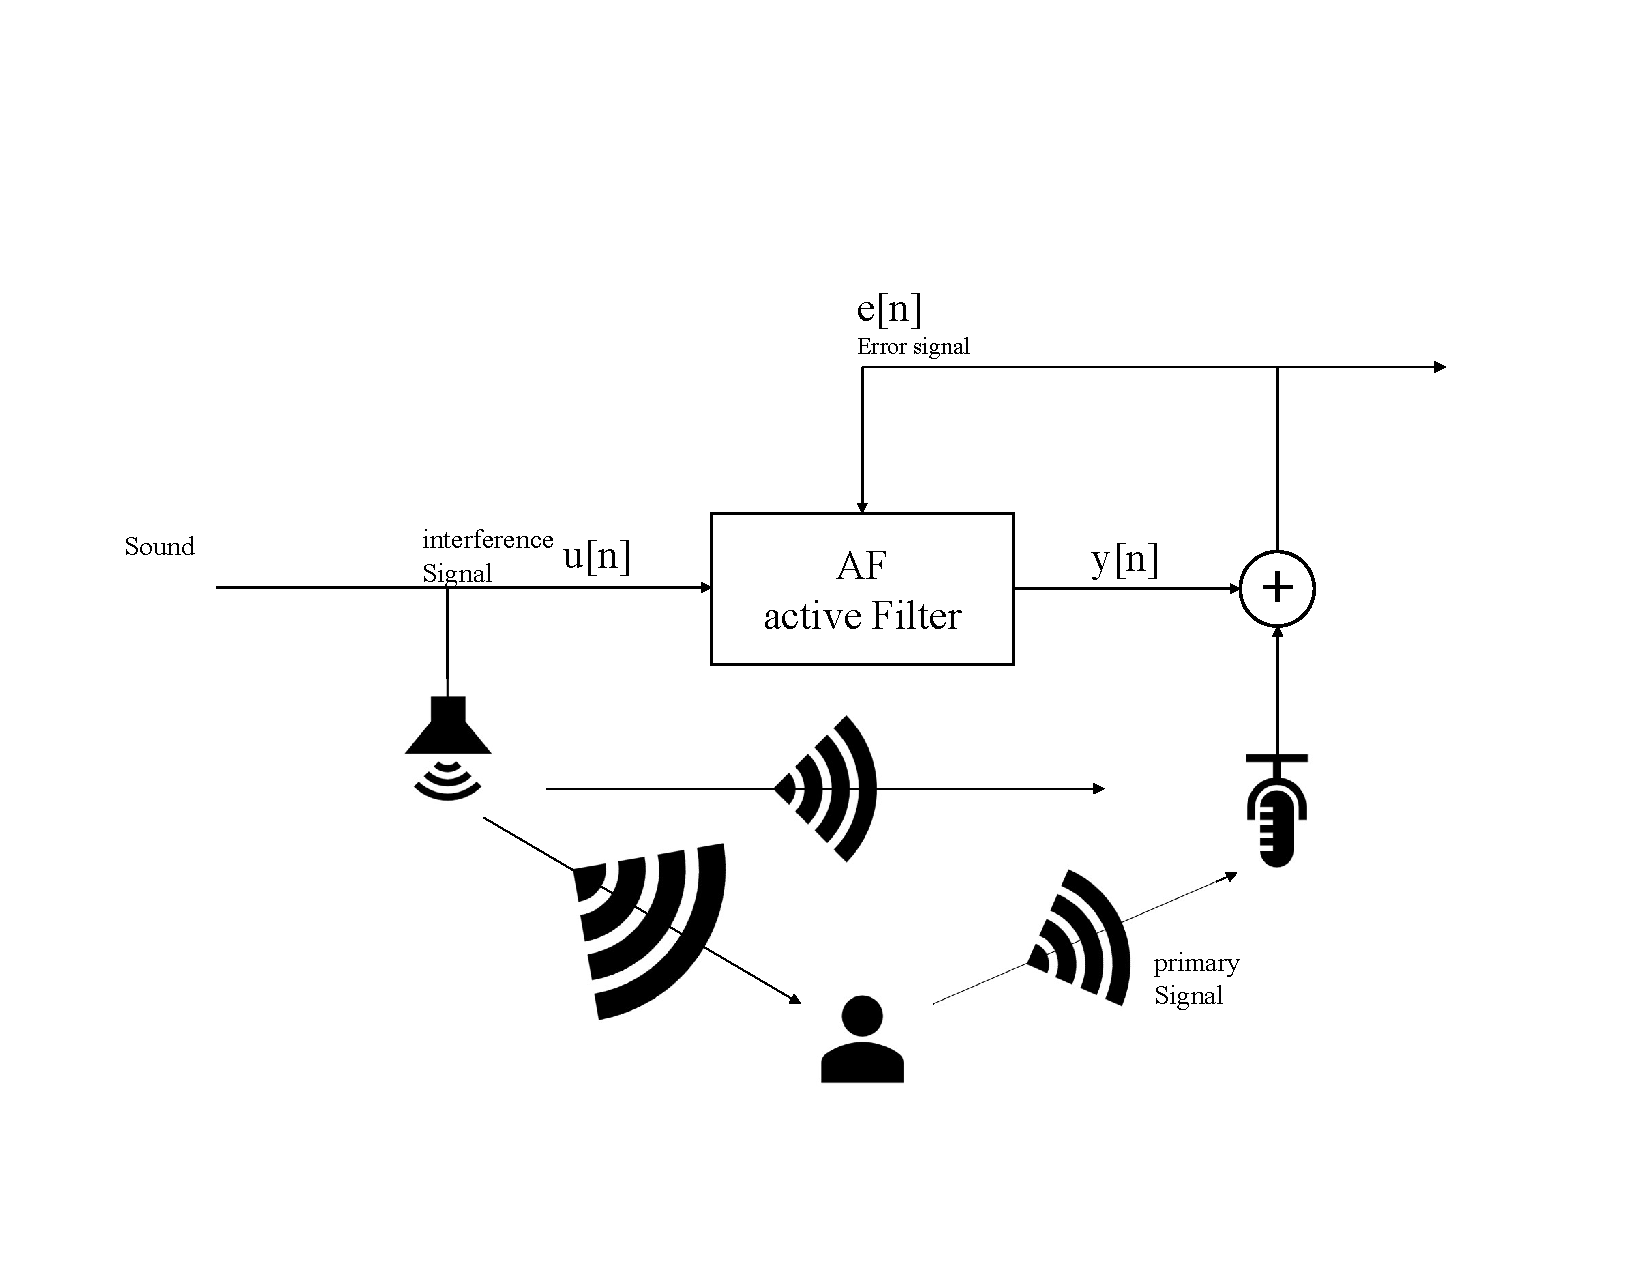
\includegraphics[scale=0.65, trim=0cm 3cm 0cm 4.5cm, clip]{interference_chanellation2.pdf}
	\caption{Example for an application for an interference-cancelling-filter}
	\label{interference2} 
\end{figure}

In Interference Cancellation - in the case of audio - the interference signal is captured and sent to the Adaptive Filter at the soundcard. Linear filters are better than nonlinear ones for this case. Filter tries to "'kill"' the interference because it knows, what has been played on the speaker.


\subsection{A Time Signal}
\null\qquad $x(t) = A(t)  cos(2  \pi  f_0  t + \varphi(t))$

\null\qquad $\varphi:=$ Phase Modulation\\
\null\qquad $A(t):=   $ Amplitude Modulation\\

- Frequency modulation is just another way of Phase Modulation. (f<->t)

\null\qquad $x(t) = \Re{u(t)  e^{j 2  \pi  f_0  t}}$

with   
\begin{itemize}
	\item $x(t)\in \mathbb{R}$: Real Signal
	\item $u(t)\in \mathbb{R}$: Complex Envelope of $x(t)$
	\item $f_0$: Center of Frequency; \quad $[f_0]=1 Hz$
\end{itemize}

Notation with Magnitude and phase:

\null\qquad $u(t)=|u(t)|\cdot e^{j\varphi_u(t)}$

\null\qquad $x(t) \iff u(t)$ 
\null\qquad\pfeil It's not a fourier transform, but related. Are different representations of the same thing. 


\null\qquad $ x(t-T) \iff u(t-T) e^{-j2 \pi \varphi T}$\\
\null\qquad $ a \in R $ \pfeil $ a \cdot x(t-T) = u(t-T) \cdot e^{-j 2 \pi \varphi^{}_{0} T} \cdot a= w^{*} \cdot u(t-T)$\\
\null\qquad $ w\ast \in \mathbb{C} \pfeil w^{*} = e^{-j 2 \pi \varphi^{}_{0} T} a$\\


\subsection{Constraints for Bandwidth}

\null\qquad $-2f_0+\frac{B}{2} \leq -\frac{B}{2} $ 

\mybox{
\pfeil  $B \leq 2 f_0$ \qquad or \qquad $f_0 \geq \frac{B}{2}$}


\begin{figure}[H]
	\centering
	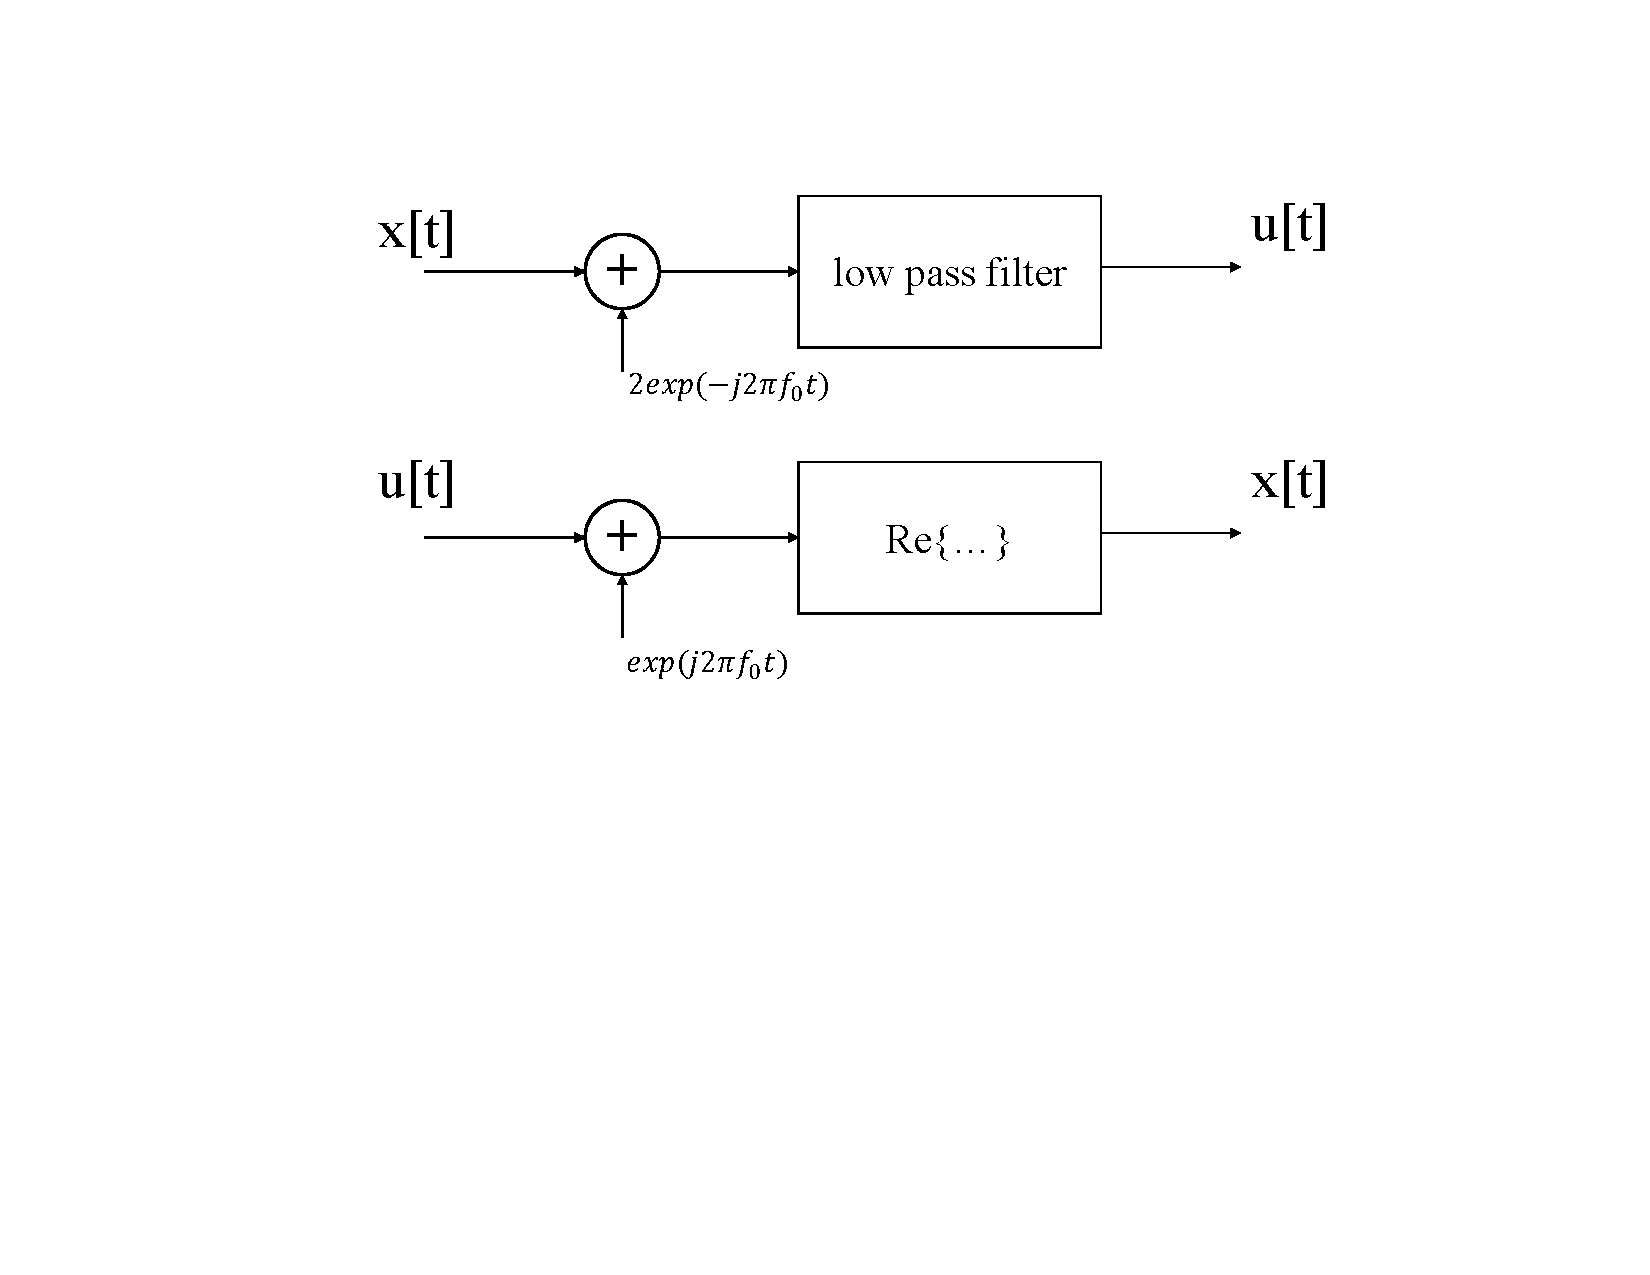
\includegraphics[scale=0.65, trim=0cm 10cm 0cm 3cm, clip]{bandpass_not_overlapping.pdf}
	\caption{Transformation from complex envelope and signal as block diagram and vice versa}
	\label{complexEnvelopTransform} 
\end{figure}

\subsection{Narrow Band}

Assumption:\\

\mybox{
	$ u(t-1/f_0) \approx u(t) $\\
	$ f_0 \triangle t = ( (\varphi w)/(2\pi) - f_0 \tau) \textit{mod}(1)$\\
	$ \triangle t = ( (\varphi w)/(2\pi f_0) - \tau) \textit{mod}(1/f_0) $
}\\

then...\\

\mybox{
	\~{t} $= ((\varphi w)/(2\pi f_0) - \tau)  \textit{mod}(1/f_0) $\\
	$ c = |w| $ := Complex envelope (only narrow bands)
}

\null\qquad $f_0$ :=  Carrier Frequency

\null\qquad $abs(w) x(t-T-\triangle t) \iff w^* u(t-T)$
\null\qquad $\triangle t = (avg(w)/(2 \pi f_0) - T) mod(1/f_0)$


\subsection{Planar Waves}
\begin{figure}[H]
	\centering
	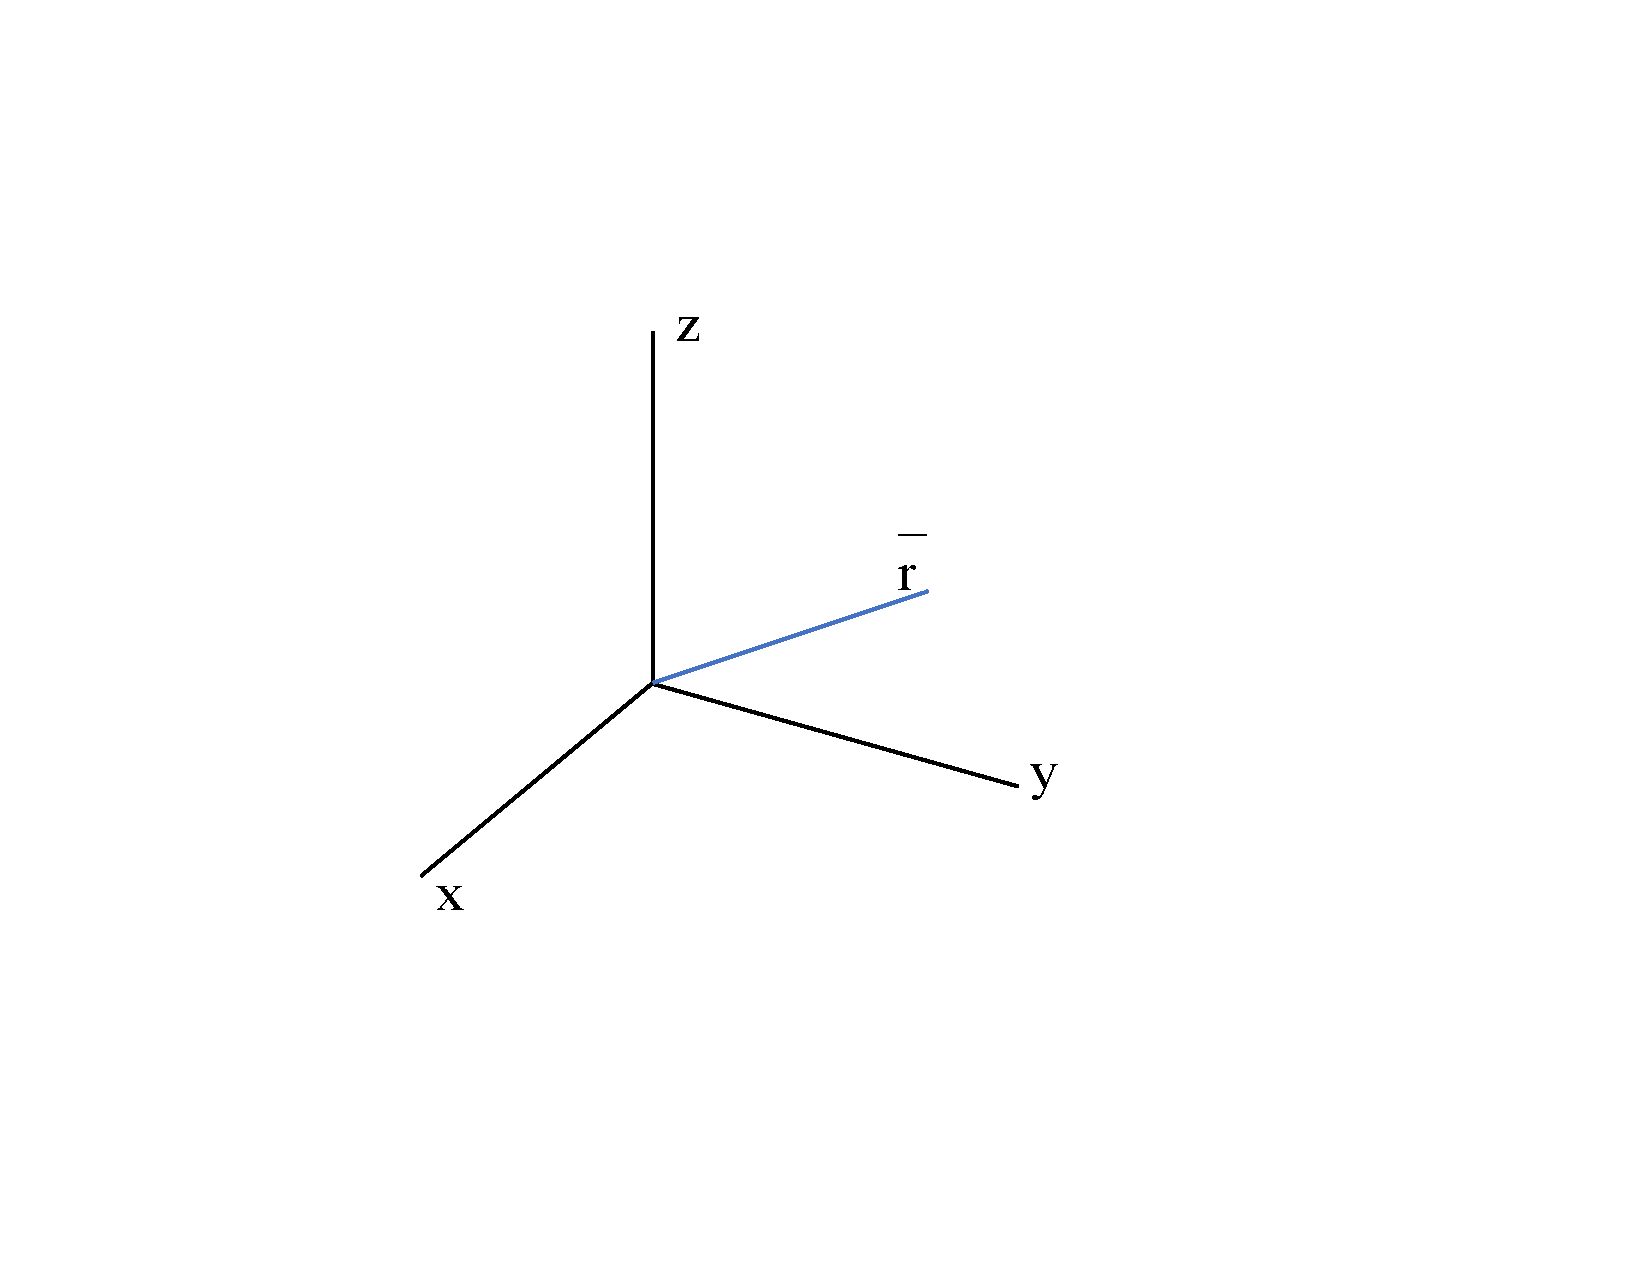
\includegraphics[scale=0.65, trim=0cm 5cm 0cm 4cm, clip]{planarwave.pdf}
	\caption{Direction of planar wave}
	\label{planarwave} 
\end{figure}


\pfeil A wave is relationship of time and space

\null\qquad $ P(t,\vecp{r}) = F(t- \vecp{n}*\vecp{r}/c) $\\
\null\qquad\pfeil \vecp{n} := unit vector \vecp{n}*\vecp{n}=1\\
\null\qquad\pfeil c > 0    := Wave Propagation Speed \\
\null\qquad\pfeil $\triangle\vecp{r}*\vecp{n} = 0$\\

\null\qquad $ P(t, \vecp{r}) = p(t, \vecp{r}+\triangle\vecp{r}) $

\textbf{Property 1}\\
$\forall \Delta \vecp{r}: \Delta \vecp{r} \cdot \vecp{n} = 0 \quad \pfeil q(t,\vecp{r}+\Delta \vecp{r})= q(t,\vecp{r})$\\
\begin{figure}[H]
	\centering
	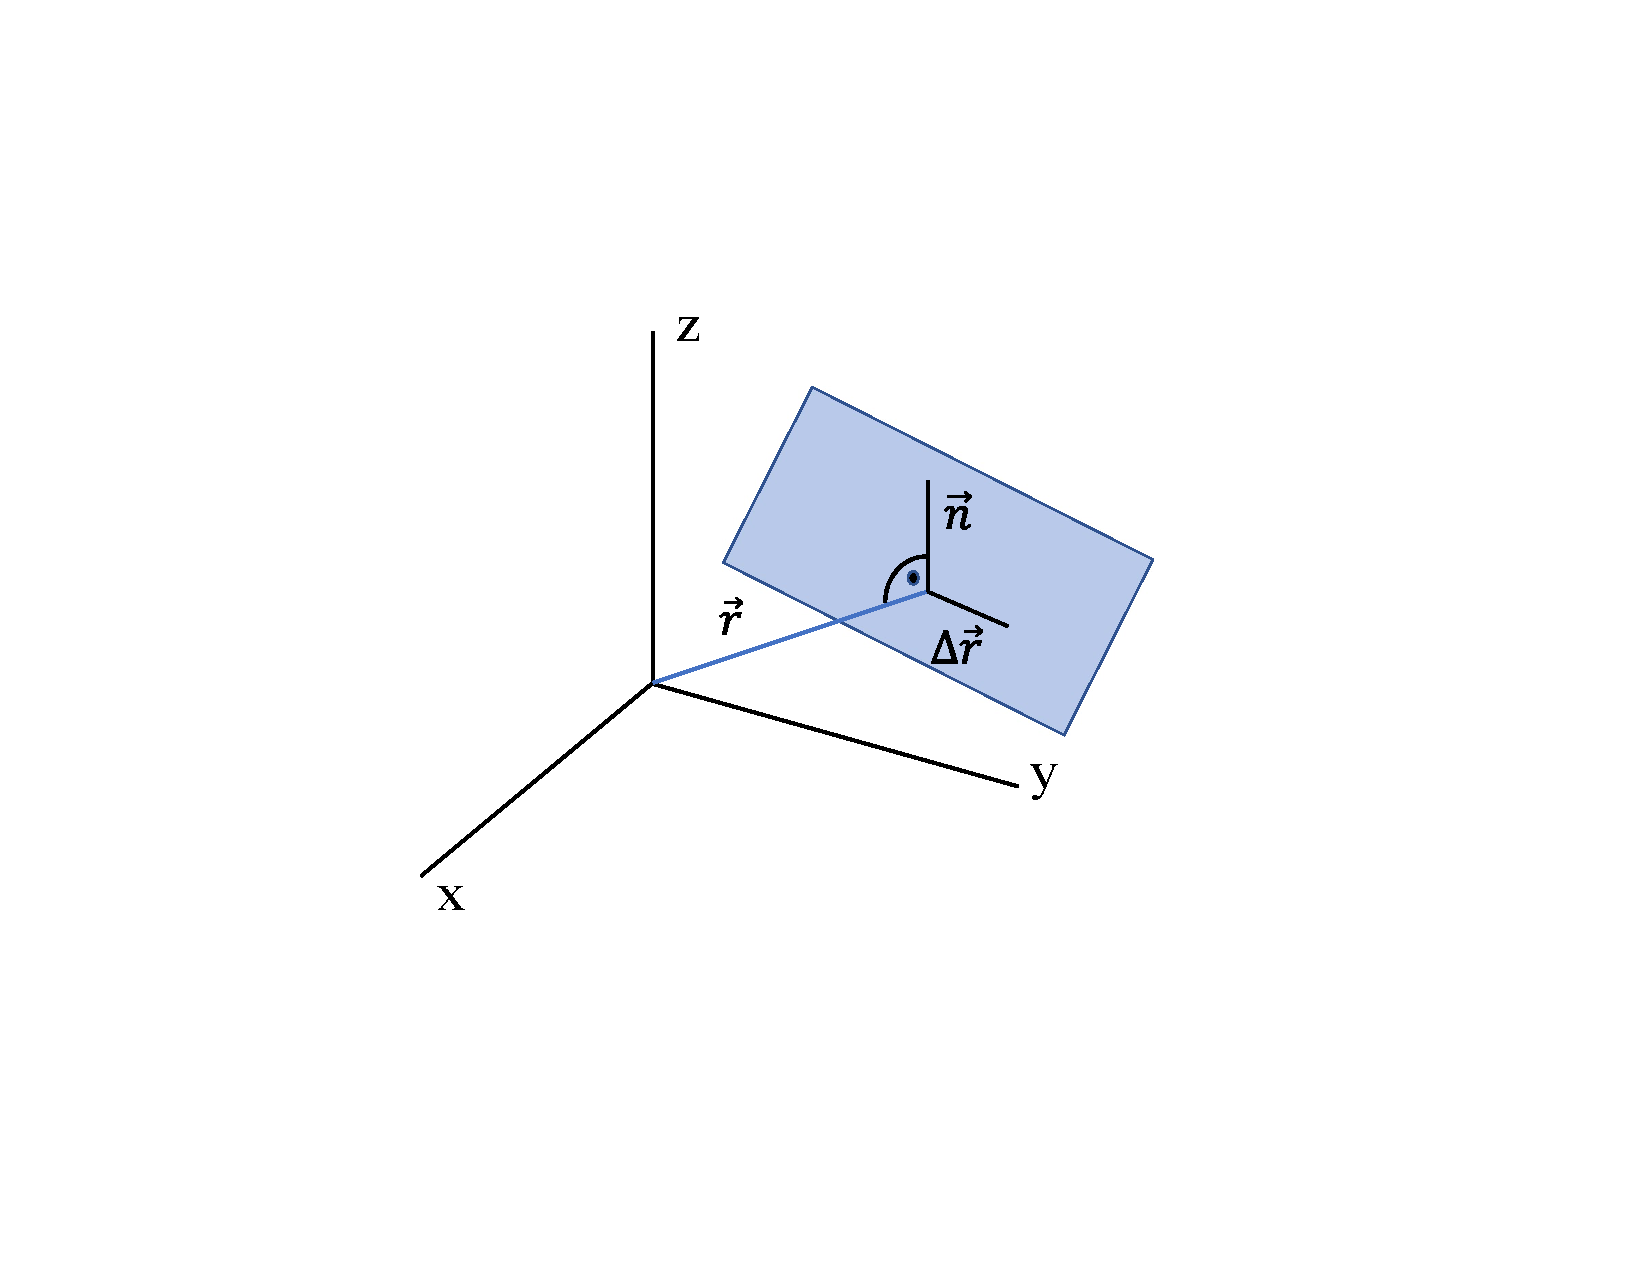
\includegraphics[scale=0.65, trim=0cm 5cm 0cm 4cm, clip]{plane.pdf}
	\caption{plane in space}
	\label{plane} 
\end{figure}

\textbf{Property 2}\\
$q(t+\Delta t, \vecp{r} + \Delta t\cdot c \vecp{n}) \equiv q(t,\vecp{r})$\\
Moving of $q(t,\vecp{r})$ into direction of $\vecp{n}$ with speed $c$.\\


\subsubsection{Harmonic Waves}
Harmonic planar waves have a third property. A harmonic wave has 

$ F(t) = A cos(2 \pi f_0 t + \varphi)$ \pfeil all const apart of t \\
$ P(t, \vecp{r}) = A cos(2 \pi f_0 (t - (\vecp{n}*\vecp{r})/c)+\varphi)$\\
\null\qquad \pfeil complex envelope\\
\null\qquad $ = \Re{u(\vecp{r})\cdot e^{j 2 \pi f_0 t}}$\\

$ u(\vecp{r}) = A e^{-j 2 \pi f_0 (\vecp{n}*\vecp{r})/c)} + e^{j\varphi} $\\ 
$ u(\vecp{r}) = A e^{j \varphi} \cdot e^{-j 2 \pi f_0 (\vecp{n}*\vecp{r})/c)} $\\
\null\qquad \pfeil $A e^{j \varphi} \in \mathbb{C} $ we call it $s$

\textbf{Property 3}
This property is only for harmonic plane waves \\


\null\qquad \pfeil $\mathbb{C}$-Envelope: 
$u(\vecp{r}+ \frac{c}{f_0}\vecp{n})\equiv u(\vecp{r})$ \qquad $\lambda$ wave length; $\lambda =\frac{c}{f_0} $\\ \ \\
\null\qquad \pfeil $u(\vecp{r}) = s\cdot  e^{-j2\pi \frac{\vecp{n}\cdot\vecp{r}}{\lambda}}$\\ \ \\

\subsection{Spatial Sampling}

\begin{figure}[H]
	\centering
	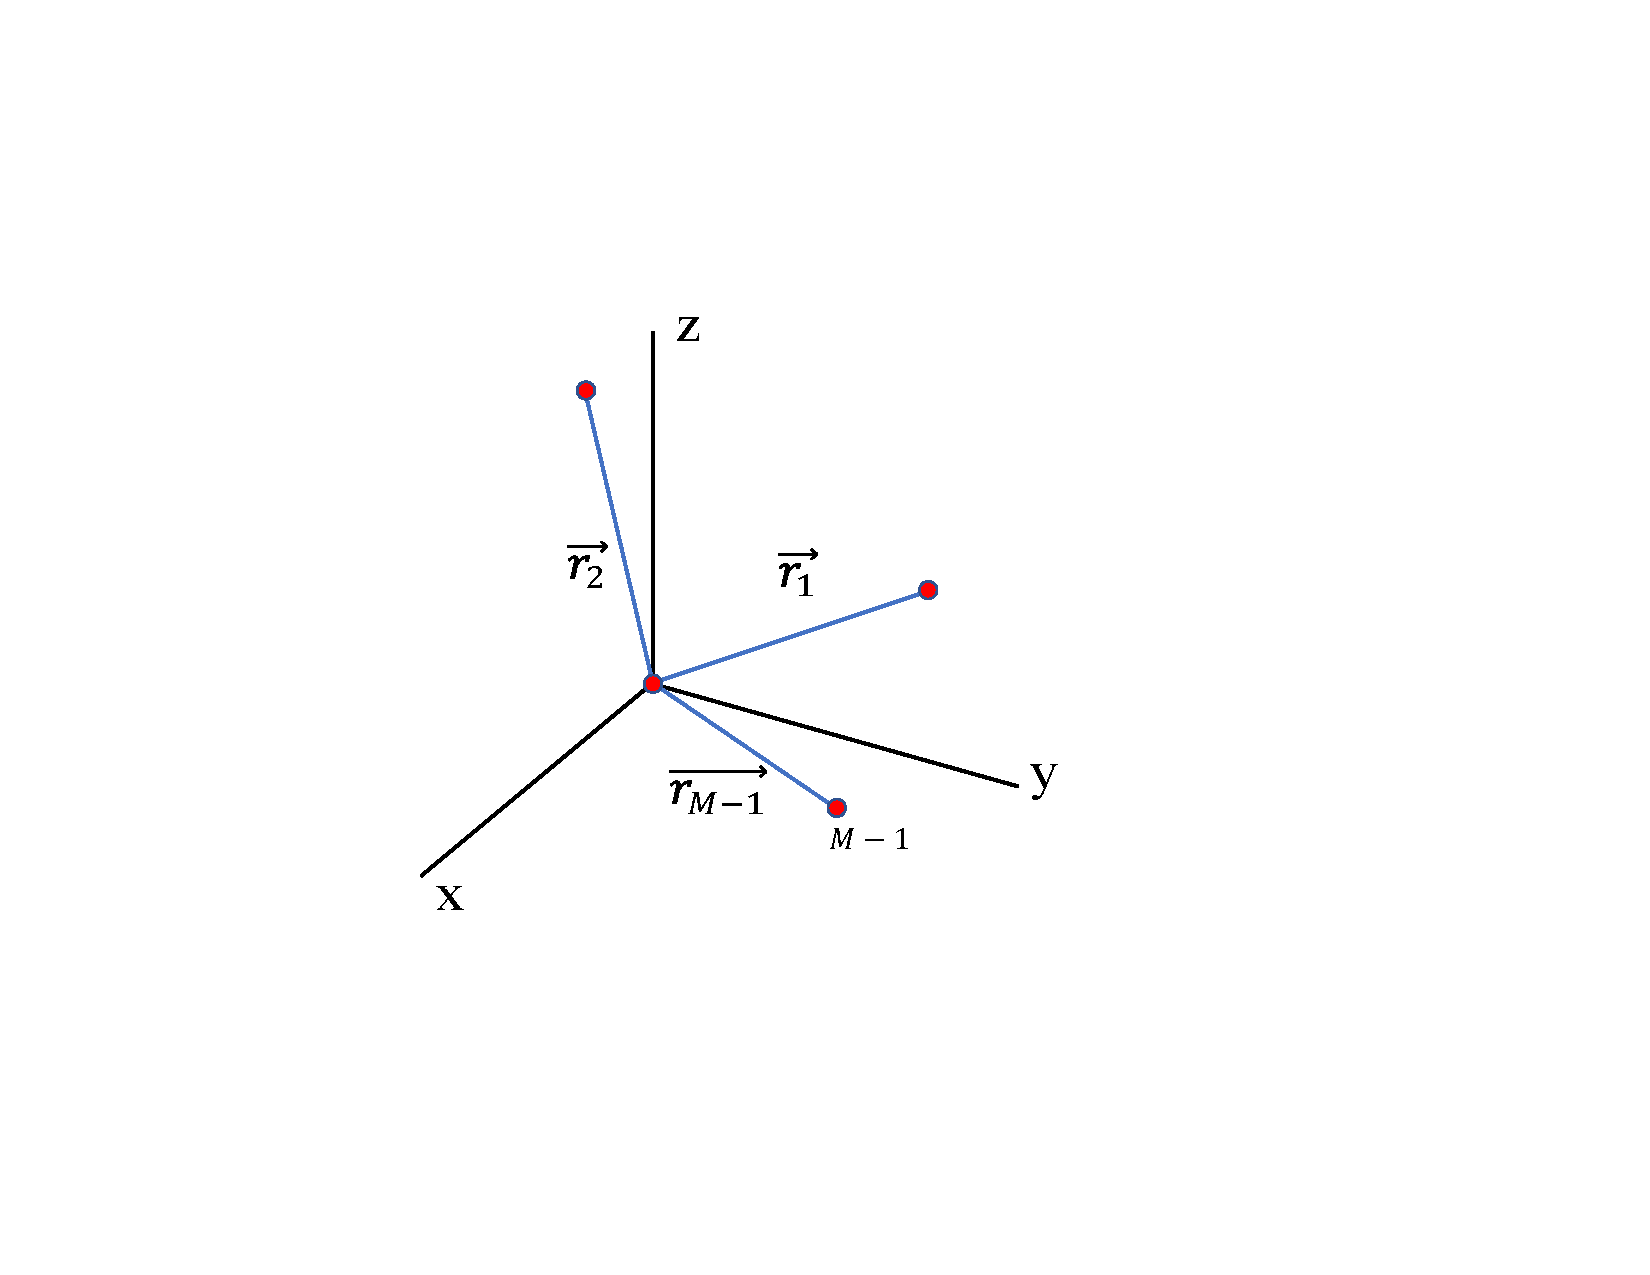
\includegraphics[scale=0.65, trim=0cm 6cm 0cm 5cm, clip]{spatialsampling.pdf}
	\caption{Spatial Sampling with M sensors}
	\label{sampling} 
\end{figure}
$\vec{u}[t]= \left[\begin{array}{c}
s(t)\\ s(t-\frac{\vecp{n}\cdot\vecp{r}_1}{c})e^{-j2\pi \frac{\vecp{n}\cdot \vecp{r}_1}{\lambda}}\\ \svdots \\s(t-\frac{\vecp{n}\cdot \vecp{r}_{M-1}}{c})e^{-j2\pi \frac{\vecp{n}\cdot \vecp{r}_{M-1}}{\lambda}} 
\end{array}\right] $\pfeil Sensor array (receive vector)\\ \ \\
Definition coherence: Coherence (physics), an ideal property of waves that enables stationary (i.e. temporally and spatially constant) interference.
